\section{Abwägung des Einsatzes eines Informationsmanagers an der Hochschule Emden Leer}
Das Soll-Konzept analysiert die Ist-Situation um festzustellen, ob es generell einer Verbesserung des Informationsmanagements bedarf und wo diese anzusetzen sind oder ob noch kein Informationsmanagement besteht und aufgebaut werden muss. Dazu sind verschiedene Aspekte zu beleuchten. Neben der Anforderung des Marketings und neben den  technischen Neuerungen und Umsetzungen ist zu klären, wer die strategische und operative Führung übernehmen soll. 

Im klassischen Informationsmanagement ist dies die Aufgabe eines Informationsmanager oder des sogenannten Chief Information Officers. Der Informationsmanager dient dabei als zentrale Schnittstelle zwischen technischen, organisatorischen und wirtschaftlichen Teilbereichen und dient dort als sogenannter Mittler und untersucht dafür die Informations- und Kommunikationstechniken in allen unterschiedlichen Bereichen um diese sinnvoll einzusetzen.\footnote{\cite[86]{krcmar_einfuhrung_2015}}

\begin{figure}[h!]
	\centering
	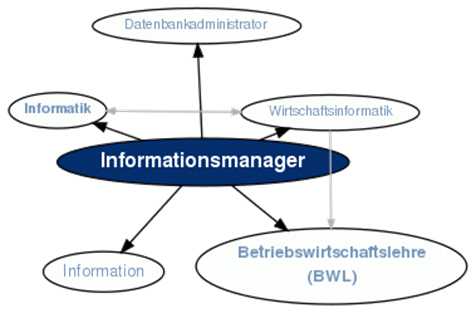
\includegraphics[width=10cm]{kapitel/gruppe3/bilder/definition_informationsmanager}
	\caption{Definition Informationsmanager}
	\label{fig_definition_informationsmanager}
\end{figure}

\subsection{Analyse des Ist-Zustandes}
Bezug nehmend auf die Abbildung \ref{fig_organigramm_HS} und der festgestellten Ist-Analyse ist festzuhalten, dass der Hochschule Emden kein Informationsmanagement im klassischen Sinne zugrunde liegt, sondern ein zentrales Informationssystem.

Es werden verschiedene Dienste und Möglichkeiten wie Moodle, Eduroam zur Verfügung gestellt und in Anspruch genommen.

Es gibt keine Verwaltung, sondern verschiedene Bereiche, die unterteilt sind in Arbeitsgruppen, Abteilungen sowie Rechenstelle und Pressestelle.

Weiterhin beinhaltet das Informationssystem verschiedene Prozesse zum 
Datenaustausch, bzw. Datenfluss 
und Backuptransfer  aus verschiedenen Systemen.\footnote{Ist-Situation \#8}

Die Nutzung des gegenwärtigen Informationssystems wird unterschiedlich stark genutzt oder ausgelastet.

Von den zentralen Einrichtungen nehmen das Hochschulrechenzentrum und die Bibliothek einen wichtigen Platz in der Hochschule ein. Das Hochschulrechenzentrum übernimmt derweil viele Aufgaben der Informationsverwaltung und Planung.

Doch nicht nur da werden Informationen gesammelt und ausgewertet. Die 
Hochschule in Emden definiert eine ganze Reihe von Arbeitsgruppen, 
beispielsweise die Arbeitsgruppe Zahlen, Daten, Fakten, die Kennzahlen der 
Hochschule und der einzelnen Fachbereiche sammelt und diese 
auswertet.\footnote{Ist-Situation \#8}

Aktuell besteht keine erweiterte Vernetzung verschiedener Intranet-Systeme 
zwischen verschiedenen Hochschulen, lediglich im Bereich der Bibliothek 
werden Inhalte an verschiedenen Standorten gemeinsam genutzt. 
Abschließend ist zu erwähnen, dass die Hochschule Emden auch keine 
einzelne Person oder ein Gremium  als Informationsmanager besitzt.

\subsection{Analyse des zu erwartenden Soll-Zustandes}
Nach Betrachtung der Best-Practice Beispiele anderer Hochschulen, lässt sich erkennen, dass jede Hochschule und auch Universität den Umgang des Informationsmanagements anders angeht. So spielen verschiedene Faktoren eine Rolle, die an jeder Hochschule unterschiedlich ausgelegt sind.

Ein Vergleich der betrachteten Hochschulen mit der Hochschule Emden zeigt, dass Emden eine wesentlich kleinere Hochschule ist und somit andere Ansprüche sowie nicht so komplexe Strukturen besitzt, als beispielsweise die WWU Münster, die über 40.000 Studierende pflegt.

Trotz unterschiedlich integrierter Möglichkeiten zur Umsetzung des jeweiligen Informationsmanagements, gibt es doch Bereiche die gleich oder relativ ähnlich sind. So sind Bibliotheken, Gremien, Ausschüsse, ebenso wie Fachbereiche und auch das Präsidium Teil einer jeden Hochschule oder Universität.

Es ist zu schauen wo sich das Informationsmanagement ansetzen lässt um mehrere Bereiche und Bestandteile untereinander zu verbinden. Fakt ist, dass es in Emden bereits Arbeitsgruppen gibt, die bestimmte Informationen gewinnen und filtern. So wäre der Aufbau einer neuen Struktur eine Möglichkeit zur Verbesserung des Informationsaustausches.

In Abschnitt \ref{subsection_zentralisierung_integration} (Zentralisierung/Integration) wird beschrieben, dass in den meisten Hochschulen viele Bestandteile unter einer Organisation arbeiten. In den meisten Fällen sind dies das Rechenzentrum, die Bibliothek und die Verwaltung.

\subsubsection{Verschiedene Empfehlungen der ZKI}
Neben verschiedenen Projekten und Einrichtungen, die sich an Hochschulen um das 
Informationsmanagement kümmern und es leiten, gibt es unter anderem noch die Zentren 
für Kommunikation und Informationsverarbeitung in Lehre und Forschung, die Empfehlungen 
für Informationsmanagement gibt.

Blickend auf die Publikation der ZKI basierend auf einer Studie der CIOs und IT-Governance 
an deutschen Hochschulen aus dem Jahre 2014 wurden über mehrere Jahre hinweg folgende 
Empfehlungen für Hochschulen ausgesprochen.

Zwischen 2001 – 2005 gab die KfR folgende Empfehlung:

\textit{Aufgrund der Relevanz der Informationsverarbeitung für alle Bereiche der  Hochschule wird empfohlen, 
	einen Generalverantwortlichen für Information und  Kommunikation (CIO, Chief Information Officer) 
	in der Hochschulleitung oder ein geeignetes Leitungsgremium mit entsprechenden 
	Entscheidungskompetenzen mit der Entwicklung und  Koordinierung aller IuK-Aufgaben 
	zu betrauen.}\footnote{\cite[3]{lang_cios_2014}}

Zwischen 2006 – 2010 werden weitere Ausführungen genannt:

\textit{„Integriertes Informationsmanagement ist daher zur wesentlichen Aufgabe bei der Planung des 
	Einsatzes moderner Techniken von Information und Kommunikation für die Hochschulen geworden. 
	Eine solche Planung setzt die Position eines Verantwortlichen für Information und Kommunikation 
	als Mitglied der Hochschulleitung (CIO: Chief Information Officer) voraus, wie er in der Wirtschaft 
	und an verschiedenen Hochschulen bereits etabliert ist.“}\footnote{\cite[16]{lang_cios_2014}}

Die KfR Empfehlungen zwischen 2011-2015 werden noch weiter ausgebaut:

\textit{„In der Hochschulpraxis lassen sich vier unterschiedliche Umsetzungstypen beobachten:  Strategischer CIO mit Leitungsfunktion: Ein Vizepräsident – oder eine Vizepräsidentin – ist explizit für das Informationsmanagement zuständig. Teilweise übernimmt auch der Kanzler die Zuständigkeit für das Informationsmanagement.}

	\begin{itemize}
		\item \textit{Strategischer CIO mit Stabsfunktion: Ein Hochschullehrer oder IT-Manager – 
			bzw. Hochschullehrerin/IT-Managerin – im Präsidialstab koordiniert das Informationsmanagement.} 
		\item \textit{Operativer CIO: Der Leiter – bzw. die Leiterin – einer zentralen 
			Informationsinfrastruktureinrichtung fungiert gleichzeitig als CIO der Hochschule.}
	    \item \textit{Kollektiver CIO: Die CIO-Funktion wird von einem Lenkungsausschuss mit zwei bis 
	    	drei Personen ausgeübt, der allerdings – anders als die traditionelle Senatskommission – über 
	    	unmittelbare Entscheidungsbefugnisse verfügt.}
	\end{itemize}
	\textit{Jede dieser CIO-Umsetzungsvarianten hat ihre Vor- und Nachteile. Es hängt von den 
		Gegebenheiten an den Hochschulen und insbesondere auch von Personen ab, welche 
		Umsetzung die am besten geeignete ist. Wichtig ist, dass der CIO – in welcher Form 
		auch immer – einen unmittelbaren Zugang zur Hochschulleitung hat und die IT-Belange 
		der gesamten Hochschule strategisch – mit unmittelbarer Richtlinien- und 
		Entscheidungskompetenz – führt und verantwortet.“} \footnote{\cite{lang_cios_2014}}

\subsubsection{Tendenz des Informationsmanagers an der Hochschule Emden/Leer}
Erkennbar sind die Tendenzen der KfR, ein einheitliches Informationsmanagement durch die Leitung eines 
Chief Information Officers. Dabei wir aber nicht nur von der Einzelperson als Informationsmanager gesprochen. 
Entsprechende Gremien sind durchaus auch ein mögliches CIO Modell. Neben der Möglichkeit einen CIO aus 
der Privatwirtschaft zu holen, besteht auch die Möglichkeit hochschulinterne Mitarbeiter zu involvieren. 
So ist zu klären, ob die Ressourcen einer Ganztagsstelle gegeben sind um eine Einzelperson als CIO zu 
verpflichten. Hier zu kommen erhöhte Personalkosten, ebenso die Einarbeitung.

Soll das Informationsmanagement allerdings nicht nur von einer einzelnen Person betrieben werden, 
ist zu klären, wer diese Aufgabe übernehmen soll. Dazu ist immer in Vergleich zu setzen, welche 
Parameter greifen. Die Studie besagt, bezugnehmend auf die Abbildung \ref{fig_herkunft_cio_hochschulen}, 
dass die Gremienmitglieder aus ganz unterschiedlichen Bereichen der Hochschule kommen. Ist dies 
der Fall und ein Gremium wird ernannt, ist ein Arbeitsaufwand der anfallenden CIO Tätigkeiten 
auf alle Mitglieder aufgeteilt. So ist der Gesamtaufwand pro Person prozentual geringer als 
bei einer einzelnen Person, die mindestens 50\% ihrer Zeit in CIO Aufgaben investiert.

\begin{figure}
	\centering
	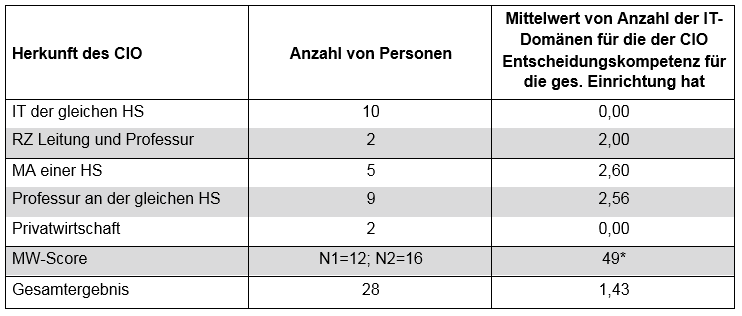
\includegraphics[width=\textwidth]
	{kapitel/gruppe3/bilder/herkunft_cio_hochschulen}
	\caption{Herkunft des CIO an verschiedenen Hochschulen, nach ZKI CIO-Studie}
	\label{fig_herkunft_cio_hochschulen}
\end{figure}

Es ist zu überlegen ob auch in Emden das Konzept eines CIO Gremium als Dachorganisation besser geeignet 
wäre als die Einstellung einer Einzelperson. So kann wie in Abbildung \ref{fig_konzept_organigramm_mit_CIO} 
gezeigt durch umstellen des Organigramms der Hochschule Emden aus verschiedenen Bereichen ein 
Gremium gebildet werden, dass die Aufgaben des CIO übernimmt und aufteilt. Mitglieder können aus 
dem Hochschulrat, den einzelnen Fachbereichen, einem Mitglied aus den Hochschulgremien, 
dem Hochschulrechenzentrum und der Bibliothek ein Gremium gebildet werden.

Anlehnend an die Empfehlungen der KfR und der speziellen Bedürfnisse die jede Hochschule besitzt, 
wäre in Emden eine Mischform des CIOs anzusiedeln.

\begin{figure}[h!]
	\centering
	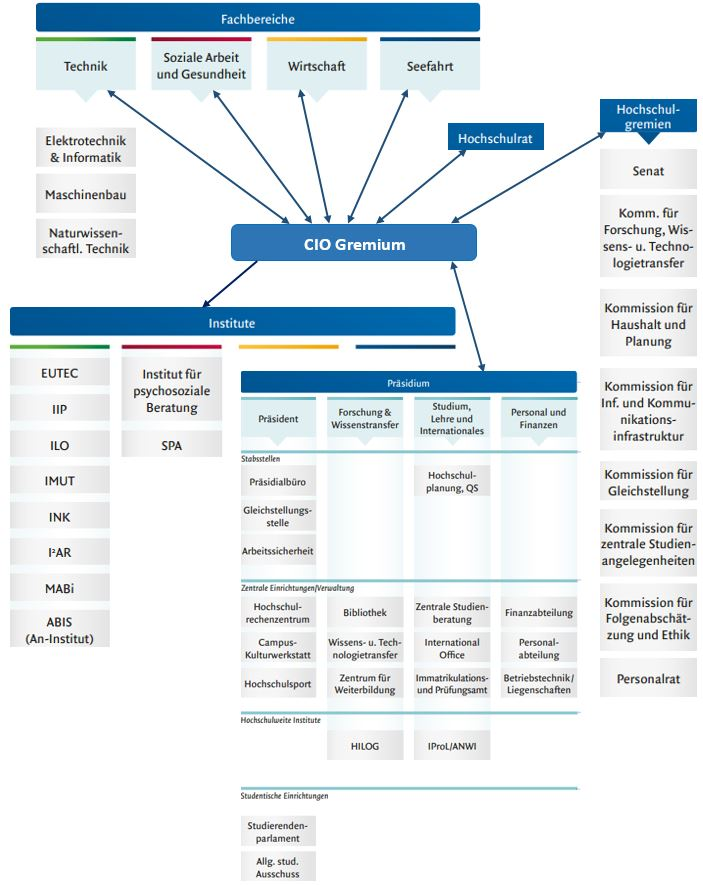
\includegraphics[width=\textwidth]
	{kapitel/gruppe3/bilder/konzept_organigramm_mit_CIO}
	\caption{Umstellung des Organigramms der Hochschule Emden hinsichtlich eines CIO Gremiums}
	\label{fig_konzept_organigramm_mit_CIO}
\end{figure}

\newpage

\subsection{Fazit}
Durch stetig wachsende technische Anforderungen und Verarbeitungen 
sowie Weitergabe von Informationen, spricht die KfR seit Jahren 
Empfehlungen bezüglich eines Informationsmanagers an Hochschulen aus. 

Durch betrachten der Best Practice Beispiele verschiedener Hochschulen wird gezeigt, 
dass jede Hochschule andere Anforderungen besitzt und bezüglich ihrer Größe, Lage und 
Ansprüche anders mit einem Informationsmanagement umgeht.

Nicht jede Lösung eignet sich dabei für jede Hochschule. 
In einer Studie der KfR geht dies ebenfalls hervor. 
Die Studie befasst sich mit dem Informationsmanagers und spricht dabei Empfehlungen für Hochschulen aus. 
Dabei ist auch wieder festzustellen, dass es neben dem Einzelpersonen- Modell auch ein CIO-Gremium Model geben kann, je nach Bedürfnis der Hochschule. 
Eine Einzelperson kann hierbei vorteilhafter sein als ein Gremium, dennoch ist zu betrachten, dass ein enormer Personeller Kosten- und Zeitfaktor entstehen wird, da nicht zu verachten ist, dass das Aufbauen einer solchen Struktur Jahre in Anspruch nimmt. 
Es ist daher abzuwägen, ob sich dieser finanzielle Aufwand lohnt.

Für die Hochschule Emden ist eine Empfehlung eines CIO Gremiums auszusprechen ,dass aus verschiedenen Bereichen eine Arbeitsgruppe bildet, die alle anfallenden CIO Aufgaben untereinander aufteilt und somit den Arbeitsaufwand prozentual auf alle aufteilt. 

Es ist anzuraten, anlehnend an die Studie der KfR eine Mischform zwischen kollektivem und strategischen CIO anzustreben.
